\documentclass{ximera}

\input{../preamble.tex}




\title{Inverse trigonometric functions}

\begin{document}
\begin{abstract}
  We introduce the inverse trigonometric functions.
\end{abstract}
\maketitle

%*** Need more in here ***

\section{What are inverse trigonometric functions?}


Trigonometric functions arise frequently in problems, and often we are
interested in finding specific angle measures. For instance, you may
want to find some angle $x$ such that
\[
\cos(x) = .7
\]
Hence we want to be able to ``undo'' trigonometric functions. However, since
trigonometric functions are not one-to-one, meaning there are are
infinitely many angles with $\cos(x) = .7$, it is impossible to
find a true inverse \emph{function} for $\cos(x)$. Nevertheless, it is
useful to have something like an inverse to these functions, however
imperfect. To do this, we restrict the domain of the trig function so that all possible output values are used exactly once; this ensures that its inverse is a function. In the case of cosine, the function $\cos(x)$ takes on all
values between $-1$ and $1$ exactly once on the interval $[0,\pi]$.

%The usual approach is to pick out some collection of angles
%that produce all possible values exactly once. If we ``discard'' all
%other angles, the resulting function has a proper inverse.  In other
%words, we are restricting the domain of the trigonometric function in
%order to find an inverse.  The function $\cos(\theta)$ takes on all
%values between $-1$ and $1$ exactly once on the interval $[0,\pi]$.

\begin{image}
\begin{tikzpicture}
	\begin{axis}[
            xmin=-6.75,xmax=6.75,ymin=-1.5,ymax=1.5,
            axis lines=center,
            xtick={-6.28, -4.71, -3.14, -1.57, 0, 1.57, 3.142, 4.71, 6.28},
            xticklabels={$-2\pi$,$-3\pi/2$,$-\pi$, $-\pi/2$, $0$, $\pi/2$, $\pi$, $3\pi/2$, $2\pi$},
            ytick={-1,1},
            %ticks=none,
            width=6in,
            height=3in,
            unit vector ratio*=1 1 1,
            xlabel=$x$, ylabel=$y$,
            every axis y label/.style={at=(current axis.above origin),anchor=south},
            every axis x label/.style={at=(current axis.right of origin),anchor=west},
          ]        
          \addplot [very thick, penColor2!20!background, samples=100,smooth, domain=(-6.75:0)] {cos(deg(x))};
          \addplot [very thick, penColor2!20!background, samples=100,smooth, domain=(3.14:6.75)] {cos(deg(x))};
          \addplot [very thick, penColor2, samples=100,smooth, domain=(0:3.14)] {cos(deg(x))};
          
          \addplot[color=penColor2,fill=penColor2,only marks,mark=*] coordinates{(0,1)};  %% closed hole          
          \addplot[color=penColor2,fill=penColor2,only marks,mark=*] coordinates{(pi,-1)};  %% closed hole          
          \node at (axis cs:-1.9,.75) [penColor2] {$y=\cos(x)$};
        \end{axis}
\end{tikzpicture}
%% \caption{The function $\cos(\theta)$ takes on all values between $-1$
%%   and $1$ exactly once on the interval $[0,\pi]$. If we restrict
%%   $\cos(\theta)$ to this interval, then this restricted function has
%%   an inverse.}
%% \label{figure:cos-restricted}
%% \end{figure*}
\end{image}
If we restrict the domain of $\cos(x)$ to this interval, then this
restricted function is one-to-one and hence has an inverse function.

\begin{question}
  What arc on the unit circle corresponds to the restricted domain
  described above of $\cos(x)$?
  \begin{multipleChoice}
    \choice{\begin{tikzpicture}[framed,scale=.2,baseline=4ex]
	\begin{axis}[
            xmin=-1.1,xmax=1.1,ymin=-1.1,ymax=1.1,
            axis lines=center,
            width=4in,
            ticks=none,
            clip=false,
            unit vector ratio*=1 1 1,
            %xlabel=$x$, ylabel=$y$,
            every axis y label/.style={at=(current axis.above origin),anchor=south},
            every axis x label/.style={at=(current axis.right of origin),anchor=west},
          ]        
          \addplot [dashed, smooth, domain=(0:360)] ({cos(x)},{sin(x)}); %% unit circle

          \addplot [line width=2mm,penColor2, domain=(-90:90)] ({cos(x)},{sin(x)}); %% unit circle
        \end{axis}
    \end{tikzpicture}}
    \choice[correct]{\begin{tikzpicture}[framed,scale=.2,baseline=4ex]
	\begin{axis}[
            xmin=-1.1,xmax=1.1,ymin=-1.1,ymax=1.1,
            axis lines=center,
            width=4in,
            ticks=none,
            clip=false,
            unit vector ratio*=1 1 1,
            %xlabel=$x$, ylabel=$y$,
            every axis y label/.style={at=(current axis.above origin),anchor=south},
            every axis x label/.style={at=(current axis.right of origin),anchor=west},
          ]        
          \addplot [dashed, smooth, domain=(0:360)] ({cos(x)},{sin(x)}); %% unit circle

          \addplot [line width=2mm,penColor2, domain=(0:180)] ({cos(x)},{sin(x)}); %% unit circle
        \end{axis}
    \end{tikzpicture}}
    \choice{\begin{tikzpicture}[framed,scale=.2,baseline=4ex]
	\begin{axis}[
            xmin=-1.1,xmax=1.1,ymin=-1.1,ymax=1.1,
            axis lines=center,
            width=4in,
            ticks=none,
            clip=false,
            unit vector ratio*=1 1 1,
            %xlabel=$x$, ylabel=$y$,
            every axis y label/.style={at=(current axis.above origin),anchor=south},
            every axis x label/.style={at=(current axis.right of origin),anchor=west},
          ]        
          \addplot [dashed, smooth, domain=(0:360)] ({cos(x)},{sin(x)}); %% unit circle

          \addplot [line width=2mm,penColor2, domain=(90:270)] ({cos(x)},{sin(x)}); %% unit circle
        \end{axis}
    \end{tikzpicture}}
    \choice{\begin{tikzpicture}[framed,scale=.2,baseline=4ex]
	\begin{axis}[
            xmin=-1.1,xmax=1.1,ymin=-1.1,ymax=1.1,
            axis lines=center,
            width=4in,
            ticks=none,
            clip=false,
            unit vector ratio*=1 1 1,
            %xlabel=$x$, ylabel=$y$,
            every axis y label/.style={at=(current axis.above origin),anchor=south},
            every axis x label/.style={at=(current axis.right of origin),anchor=west},
          ]        
          \addplot [dashed, smooth, domain=(0:360)] ({cos(x)},{sin(x)}); %% unit circle

          \addplot [line width=2mm,penColor2, domain=(180:360)] ({cos(x)},{sin(x)}); %% unit circle
        \end{axis}
\end{tikzpicture}}
  \end{multipleChoice}
\end{question}

\begin{question}
Compute the arccosine values below by finding the angle in $[0,\pi]$ whose cosine value is the input given.

\[\arccos(0)=\answer{\pi/2}\]
\[\arccos(\sqrt{2}/2)=\answer{\pi/4}\]
\[\arccos(-\sqrt{2}/2)=\answer{3\pi/4}\]
\[\arccos(-1/2)=\answer{2\pi/3}\]


\end{question}

In a similar fashion, we restrict the domain of sine to make its inverse a function. The function $\sin(x)$ takes on all values between $-1$ and $1$ exactly once on the interval $[-\pi/2,\pi/2]$.

\begin{image}
\begin{tikzpicture}
	\begin{axis}[
            xmin=-6.75,xmax=6.75,ymin=-1.5,ymax=1.5,
            axis lines=center,
            xtick={-6.28, -4.71, -3.14, -1.57, 0, 1.57, 3.142, 4.71, 6.28},
            xticklabels={$-2\pi$,$-3\pi/2$,$-\pi$, $-\pi/2$, $0$, $\pi/2$, $\pi$, $3\pi/2$, $2\pi$},
            ytick={-1,1},
            %ticks=none,
            width=6in,
            height=3in,
            unit vector ratio*=1 1 1,
            xlabel=$x$, ylabel=$y$,
            every axis y label/.style={at=(current axis.above origin),anchor=south},
            every axis x label/.style={at=(current axis.right of origin),anchor=west},
          ]        
          \addplot [very thick, penColor!20!background, samples=100,smooth, domain=(-6.75:-1.57)] {sin(deg(x))};
          \addplot [very thick, penColor!20!background, samples=100,smooth, domain=(1.57:6.75)] {sin(deg(x))};
          \addplot [very thick, penColor, samples=100,smooth, domain=(-1.57:1.57)] {sin(deg(x))};
          
          \addplot[color=penColor,fill=penColor,only marks,mark=*] coordinates{(-1.57,-1)};  %% closed hole          
          \addplot[color=penColor,fill=penColor,only marks,mark=*] coordinates{(1.57,1)};  %% closed hole          
          \node at (axis cs:3.5,.75) [penColor] {$y=\sin(x)$};
        \end{axis}
\end{tikzpicture}
%% \caption{The function $\sin(\theta)$ takes on all values between $-1$
%%   and $1$ exactly once on the interval $[-\pi/2,\pi/2]$. If we
%%   restrict $\sin(\theta)$ to this interval, then this restricted
%%   function has an inverse.}
%% \label{figure:sin-restricted}
%% \end{figure*}
\end{image}

If we restrict the domain of $\sin(x)$ to this interval, then this restricted
function is one-to-one and thus has an inverse function.

\begin{question}
  What arc on the unit circle corresponds to the restricted domain described above of
  $\sin(x)$?
  \begin{multipleChoice}
    \choice[correct]{\begin{tikzpicture}[framed,scale=.2,baseline=4ex]
	\begin{axis}[
            xmin=-1.1,xmax=1.1,ymin=-1.1,ymax=1.1,
            axis lines=center,
            width=4in,
            ticks=none,
            clip=false,
            unit vector ratio*=1 1 1,
            %xlabel=$x$, ylabel=$y$,
            every axis y label/.style={at=(current axis.above origin),anchor=south},
            every axis x label/.style={at=(current axis.right of origin),anchor=west},
          ]        
          \addplot [dashed, smooth, domain=(0:360)] ({cos(x)},{sin(x)}); %% unit circle

          \addplot [line width=2mm,penColor, domain=(-90:90)] ({cos(x)},{sin(x)}); %% unit circle
        \end{axis}
    \end{tikzpicture}}
    \choice{\begin{tikzpicture}[framed,scale=.2,baseline=4ex]
	\begin{axis}[
            xmin=-1.1,xmax=1.1,ymin=-1.1,ymax=1.1,
            axis lines=center,
            width=4in,
            ticks=none,
            clip=false,
            unit vector ratio*=1 1 1,
            %xlabel=$x$, ylabel=$y$,
            every axis y label/.style={at=(current axis.above origin),anchor=south},
            every axis x label/.style={at=(current axis.right of origin),anchor=west},
          ]        
          \addplot [dashed, smooth, domain=(0:360)] ({cos(x)},{sin(x)}); %% unit circle

          \addplot [line width=2mm,penColor, domain=(0:180)] ({cos(x)},{sin(x)}); %% unit circle
        \end{axis}
    \end{tikzpicture}}
    \choice{\begin{tikzpicture}[framed,scale=.2,baseline=4ex]
	\begin{axis}[
            xmin=-1.1,xmax=1.1,ymin=-1.1,ymax=1.1,
            axis lines=center,
            width=4in,
            ticks=none,
            clip=false,
            unit vector ratio*=1 1 1,
            %xlabel=$x$, ylabel=$y$,
            every axis y label/.style={at=(current axis.above origin),anchor=south},
            every axis x label/.style={at=(current axis.right of origin),anchor=west},
          ]        
          \addplot [dashed, smooth, domain=(0:360)] ({cos(x)},{sin(x)}); %% unit circle

          \addplot [line width=2mm,penColor, domain=(90:270)] ({cos(x)},{sin(x)}); %% unit circle
        \end{axis}
    \end{tikzpicture}}
    \choice{\begin{tikzpicture}[framed,scale=.2,baseline=4ex]
	\begin{axis}[
            xmin=-1.1,xmax=1.1,ymin=-1.1,ymax=1.1,
            axis lines=center,
            width=4in,
            ticks=none,
            clip=false,
            unit vector ratio*=1 1 1,
            %xlabel=$x$, ylabel=$y$,
            every axis y label/.style={at=(current axis.above origin),anchor=south},
            every axis x label/.style={at=(current axis.right of origin),anchor=west},
          ]        
          \addplot [dashed, smooth, domain=(0:360)] ({cos(x)},{sin(x)}); %% unit circle

          \addplot [line width=2mm,penColor, domain=(180:360)] ({cos(x)},{sin(x)}); %% unit circle
        \end{axis}
\end{tikzpicture}}
  \end{multipleChoice}
\end{question}

\begin{question}
Compute the arcsine values below by finding the angle in $[-\pi/2,\pi/2]$ whose sine value is the input given.

\[\arcsin(0)=\answer{0}\]
\[\arcsin(\sqrt{2}/2)=\answer{\pi/4}\]
\[\arcsin(-\sqrt{2}/2)=\answer{-\pi/4}\]
\[\arcsin(-1/2)=\answer{-\pi/6}\]


\end{question}

By examining both sine and cosine on restricted domains, we can now produce functions arcsine and arccosine:

\begin{image}[2in]\index{arccosine}
\begin{tikzpicture}
	\begin{axis}[
            xmin=-1.5,xmax=1.5,ymin=-.25,ymax=3.25,
            axis lines=center,
            ytick={0, 1.57,3.14},
            yticklabels={$0$, $\pi/2$,$\pi$},
            xtick={-1,1},
            unit vector ratio*=1 1 1,
            xlabel=$x$, ylabel=$y$,
            every axis y label/.style={at=(current axis.above origin),anchor=south},
            every axis x label/.style={at=(current axis.right of origin),anchor=west},
          ]        
          \addplot [very thick, penColor5, samples=100,smooth, domain=(-1:1)] {acos(x)*pi/180};
          \addplot[color=penColor5,fill=penColor5,only marks,mark=*] coordinates{(1,0)};  %% closed hole          
          \addplot[color=penColor5,fill=penColor5,only marks,mark=*] coordinates{(-1,pi)};  %% closed hole
        \end{axis}
        \node at (3,-1) [text width=2.75in] {Here we see a plot of $y=\arccos(x)$, the inverse function of
          $y=\cos(x)$ when the domain is restricted to the interval $[0,\pi]$.};
\end{tikzpicture} 
\end{image}
\begin{image}[2in]\index{arcsine}
\begin{tikzpicture}
	\begin{axis}[
            xmin=-1.5,xmax=1.5,ymin=-1.75,ymax=1.75,
            axis lines=center,
            ytick={-1.57, 0, 1.57},
            yticklabels={$-\pi/2$, $0$, $\pi/2$},
            xtick={-1,1},
            unit vector ratio*=1 1 1,
            xlabel=$x$, ylabel=$y$,
            every axis y label/.style={at=(current axis.above origin),anchor=south},
            every axis x label/.style={at=(current axis.right of origin),anchor=west},
          ]        
          \addplot [very thick, penColor4, samples=100,smooth, domain=(-1:1)] {asin(x)*pi/180};
                    
          \addplot[color=penColor4,fill=penColor4,only marks,mark=*] coordinates{(-1,-pi/2)};  %% closed hole          
          \addplot[color=penColor4,fill=penColor4,only marks,mark=*] coordinates{(1,pi/2)};  %% closed hole
        \end{axis}
        \node at (3,-1) [text width=2.75in] {Here we see a plot of $y=\arcsin(x)$, the inverse function of
$y=\sin(x)$ when the domain is restricted to the interval $[-\pi/2,\pi/2]$.};
\end{tikzpicture} 
\end{image}

%The functions
%\[
%\arccos(x)\qquad\text{and}\qquad\arcsin(x)
%\]
%are called ``arc'' because they give the angle that cosine or sine
%used to produce their value.  
It is quite common to write
\[
\arccos(x) = \cos^{-1}(x)\qquad\text{and}\qquad\arcsin(x) = \sin^{-1}(x).
\]
However, this notation is misleading as $\cos^{-1}(x)$ and
$\sin^{-1}(x)$ are not true inverse functions of cosine and sine (due to the restricted domains), nor do they correspond to the $-1$ exponent (recall that $(\sin(x))^{-1}=\dfrac{1}{\sin(x)}=\csc(x)$).
By definition a function and its inverse undo each other in either
order, for example,
\[
\sqrt[3]{x^3}=x\qquad \text{and}\qquad \left(\sqrt[3]{x}\right)^3=x. 
\]
Since arcsine is the inverse of sine \emph{restricted to the interval}
$[-\pi/2,\pi/2]$, this does not work with sine and arcsine. For
example
\[
\arcsin(\sin(\pi))=0.
\]
However, it is true that for all $x$
\[
\sin(\arcsin(x)) = x\qquad\text{and}\qquad\cos(\arccos(x)) = x.
\]
\begin{question}
   Which of the following statements is true?
   \begin{multipleChoice}
     \choice{$\sin^{-1}(x)$ is the inverse function of $\sin(x)$} %this is perhaps a bit too subtle?
     \choice[correct]{$\sin\left(\sin^{-1}\left(\frac{1}{2}\right)\right) = \frac{1}{2}$} 
     \choice{$\sin^{-1}\left(\sin\left(\frac{5\pi}{2}\right)\right) = \frac{5\pi}{2}$}
     \choice{$\sin^{-1}(x) = \frac{1}{\sin(x)}$}
   \end{multipleChoice}  
\end{question}



\begin{example}
  Compute:
  \[
  \arccos(\cos(5\pi/3))
  \]
  \begin{explanation}
    Since $5\pi/3$ is not in the range of
    arccosine, our answer is not simply $5\pi/3$. Instead, we have:
    \[  \arccos(\cos(5\pi/3))=\arccos(1/2)=\pi/3.\]
    
Alternatively, we could bypass the $1/2$ computation by recognizing that $\pi/3$ is the angle in the range of $\arccos(x)$ with the same cosine value as $5\pi/3$.
    
%    To find our missing number, we'll check with a unit
%    circle that we've decorated with the domain of arccosine:
%\begin{image}
%\begin{tikzpicture}
%	\begin{axis}[
%            xmin=-1.1,xmax=1.1,ymin=-1.1,ymax=1.1,
%            axis lines=center,
%            width=4in,
%            ticks=none,
%            clip=false,
%            unit vector ratio*=1 1 1,
%            xlabel=$x$, ylabel=$y$,
%            every axis y label/.style={at=(current axis.above origin),anchor=south},
%            every axis x label/.style={at=(current axis.right of origin),anchor=west},
%          ]        
%          \addplot [dashed, smooth, domain=(0:360)] ({cos(x)},{sin(x)}); %% unit circle
%          \addplot [very thick, color=penColor2, smooth, domain=(0:180)] ({cos(x)},{sin(x)}); %% domain
%          \addplot[color=penColor2,fill=penColor2,only marks,mark=*] coordinates{({cos(60)},{sin(60)})};  %% closed hole
%          \addplot[color=penColor2,fill=penColor2,only marks,mark=*] coordinates{({cos(120)},{sin(120)})};  %% closed hole
%          \addplot[color=penColor2,fill=penColor2,only marks,mark=*] coordinates{({cos(180)},{sin(180)})};  %% closed hole
%          \addplot[only marks,mark=*] coordinates{({cos(240)},{sin(240)})};  %% closed hole
%          \addplot[only marks,mark=*] coordinates{({cos(300)},{sin(300)})};  %% closed hole
%          \addplot[color=penColor2,fill=penColor2,only marks,mark=*] coordinates{({cos(360)},{sin(360)})};  %% closed hole
%
%          \node at (axis cs:{(1,0)}) [anchor=south west,penColor2] {$0$};
%          \node at (axis cs:{cos(60)},{sin(60)}) [anchor=south west,penColor2] {$\pi/3$};
%          \node at (axis cs:{cos(120)},{sin(120)}) [anchor=south east,penColor2] {$2\pi/3$};
%          \node at (axis cs:{cos(180)},{sin(180)}) [anchor=south east,penColor2] {$\pi$};
%          
%          \node at (axis cs:{cos(60)},{sin(60)}) [anchor=north east] {$\pi/3$};
%          \node at (axis cs:{cos(120)},{sin(120)}) [anchor=north west] {$2\pi/3$};
%          \node at (axis cs:{cos(180)},{sin(180)}) [anchor=north west] {$\pi$};
%          \node at (axis cs:{cos(240)},{sin(240)}) [anchor=south west] {$4\pi/3$};
%          \node at (axis cs:{cos(300)},{sin(300)}) [anchor=south east] {$5\pi/3$};
%          %\node at (axis cs:{cos(360)},{sin(360)}) [anchor=north east] {$2\pi$};
%        \end{axis}          
%\end{tikzpicture}
%\end{image}
%Since the points $5\pi/3$ and $\pi/3$ have the same $x$-coordinate,
%$\cos(5\pi/3) = \cos(\pi/3)$. Hence
%\[
%\arccos(\cos(5\pi/3)) = \pi/3.
%\]
  \end{explanation}
\end{example}


Now that you have a feel for how $\arcsin(x)$ and $\arccos(x)$ behave, let's examine tangent.

\begin{image}
\begin{tikzpicture}
	\begin{axis}[
            xmin=-6.75,xmax=6.75,ymin=-3,ymax=3,
            axis lines=center,
            width=6in,
            height=3in,
            xtick={-6.28, -4.71, -3.14, -1.57, 0, 1.57, 3.142, 4.71, 6.28},
            xticklabels={$-2\pi$,$-3\pi/2$,$-\pi$, $-\pi/2$, $0$, $\pi/2$, $\pi$, $3\pi/2$, $2\pi$},       
            unit vector ratio*=1 1 1,
            xlabel=$x$, ylabel=$y$,
            every axis y label/.style={at=(current axis.above origin),anchor=south},
            every axis x label/.style={at=(current axis.right of origin),anchor=west},
          ]        
          \addplot [very thick, penColor3, samples=100,smooth, domain=(-1.55:1.55)] {tan(deg(x))};
          \addplot [very thick, penColor3!30!background, samples=100,smooth, domain=(-4.69:-1.59)] {tan(deg(x))};
          \addplot [very thick, penColor3!30!background, samples=100,smooth, domain=(-6.75:-4.73)] {tan(deg(x))};
          \addplot [very thick, penColor3!30!background, samples=100,smooth, domain=(1.59:4.69)] {tan(deg(x))};
          \addplot [very thick, penColor3!30!background, samples=100,smooth, domain=(4.73:6.75)] {tan(deg(x))};
          
          \addplot [textColor,dashed] plot coordinates {(-4.71,-3) (-4.71,3)};
          \addplot [textColor,dashed] plot coordinates {(-1.57,-3) (-1.57,3)};
          \addplot [textColor,dashed] plot coordinates {(1.57,-3) (1.57,3)};
          \addplot [textColor,dashed] plot coordinates {(4.71,-3) (4.71,3)};
          
          \node at (axis cs:0,1.25) [penColor3] {$y=\tan(x)$};    
        \end{axis}
\end{tikzpicture}
%% \caption{The function $\tan(\theta)$ takes on all values in $\R$
%%   exactly once on the open interval $(-\pi/2,\pi/2)$. If we restrict
%%   $\tan(\theta)$ to this interval, then this restricted function has
%%   an inverse.}
%% \end{figure*}
%% \end{fullwidth}
\end{image}
  \begin{question}
  What arc on the unit circle corresponds to the restricted domain described above of
  $\tan(x)$?
  \begin{multipleChoice}
    \choice[correct]{\begin{tikzpicture}[framed,scale=.2,baseline=4ex]
	\begin{axis}[
            xmin=-1.1,xmax=1.1,ymin=-1.1,ymax=1.1,
            axis lines=center,
            width=4in,
            ticks=none,
            clip=false,
            unit vector ratio*=1 1 1,
            %xlabel=$x$, ylabel=$y$,
            every axis y label/.style={at=(current axis.above origin),anchor=south},
            every axis x label/.style={at=(current axis.right of origin),anchor=west},
          ]        
          \addplot [dashed, smooth, domain=(0:360)] ({cos(x)},{sin(x)}); %% unit circle

          \addplot [line width=2mm,penColor3, domain=(-90:90)] ({cos(x)},{sin(x)}); %% unit circle
        \end{axis}
    \end{tikzpicture}}
    \choice{\begin{tikzpicture}[framed,scale=.2,baseline=4ex]
	\begin{axis}[
            xmin=-1.1,xmax=1.1,ymin=-1.1,ymax=1.1,
            axis lines=center,
            width=4in,
            ticks=none,
            clip=false,
            unit vector ratio*=1 1 1,
            %xlabel=$x$, ylabel=$y$,
            every axis y label/.style={at=(current axis.above origin),anchor=south},
            every axis x label/.style={at=(current axis.right of origin),anchor=west},
          ]        
          \addplot [dashed, smooth, domain=(0:360)] ({cos(x)},{sin(x)}); %% unit circle

          \addplot [line width=2mm,penColor3, domain=(0:180)] ({cos(x)},{sin(x)}); %% unit circle
        \end{axis}
    \end{tikzpicture}}
    \choice{\begin{tikzpicture}[framed,scale=.2,baseline=4ex]
	\begin{axis}[
            xmin=-1.1,xmax=1.1,ymin=-1.1,ymax=1.1,
            axis lines=center,
            width=4in,
            ticks=none,
            clip=false,
            unit vector ratio*=1 1 1,
            %xlabel=$x$, ylabel=$y$,
            every axis y label/.style={at=(current axis.above origin),anchor=south},
            every axis x label/.style={at=(current axis.right of origin),anchor=west},
          ]        
          \addplot [dashed, smooth, domain=(0:360)] ({cos(x)},{sin(x)}); %% unit circle

          \addplot [line width=2mm,penColor3, domain=(90:270)] ({cos(x)},{sin(x)}); %% unit circle
        \end{axis}
    \end{tikzpicture}}
    \choice{\begin{tikzpicture}[framed,scale=.2,baseline=4ex]
	\begin{axis}[
            xmin=-1.1,xmax=1.1,ymin=-1.1,ymax=1.1,
            axis lines=center,
            width=4in,
            ticks=none,
            clip=false,
            unit vector ratio*=1 1 1,
            %xlabel=$x$, ylabel=$y$,
            every axis y label/.style={at=(current axis.above origin),anchor=south},
            every axis x label/.style={at=(current axis.right of origin),anchor=west},
          ]        
          \addplot [dashed, smooth, domain=(0:360)] ({cos(x)},{sin(x)}); %% unit circle

          \addplot [line width=2mm,penColor3, domain=(180:360)] ({cos(x)},{sin(x)}); %% unit circle
        \end{axis}
\end{tikzpicture}}
  \end{multipleChoice}
\end{question}
Again, only working on a restricted domain of tangent, we can produce
an inverse function, arctangent. Here we see a plot of $y=\arctan(x)$, also written $\tan^{-1}(x)$,
the inverse function of $y=\tan(x)$ when its domain is restricted to the
interval $(-\pi/2,\pi/2)$.

\begin{image}
\begin{tikzpicture}
	\begin{axis}[
            xmin=-6,xmax=6,ymin=-2,ymax=2,
            axis lines=center,
            ytick={0, -1.57,1.57},
            width=6in,
            height=3in,
            yticklabels={$0$, $-\pi/2$,$\pi/2$},
            xtick={0},
            unit vector ratio*=1 1 1,
            xlabel=$x$, ylabel=$y$,
            every axis y label/.style={at=(current axis.above origin),anchor=south},
            every axis x label/.style={at=(current axis.right of origin),anchor=west},
          ]        
          \addplot [very thick, penColor3!20!penColor2, samples=100,smooth, domain=(-6:6)] {atan(x)*pi/180};
          \addplot [textColor,dashed] plot coordinates {(-6,-1.57) (6,-1.57)};
          \addplot [textColor,dashed] plot coordinates {(-6,1.57) (6,1.57)};
        \end{axis}
\end{tikzpicture}
%% \caption{Here we see a plot of $\arctan(y)$, the inverse function of
%% $\tan(\theta)$ when it is restricted to the interval $(-\pi/2,\pi/2)$.}
%% \end{figure*}
%% \index{arctangent}
%% \end{fullwidth}
\end{image}

Notice that our three inverse trig functions thus far all appear to be continuous on their domains. This can be proven, although we omit the proofs here.

Also notice that while $\displaystyle\lim_{x\rightarrow\pm\infty}\arccos(x)$ and $\displaystyle\lim_{x\rightarrow\pm\infty}\arcsin(x)$ do not exist due to their limited domains, from the above graph we see that
\[\displaystyle\lim_{x\rightarrow\infty}\arctan(x)=\pi/2\]
and 
\[\displaystyle\lim_{x\rightarrow-\infty}\arctan(x)=-\pi/2.\]

\begin{example}
Compute \[\displaystyle\lim_{x\rightarrow\infty}\arctan(e^x) \mbox{  and  }\displaystyle\lim_{x\rightarrow 0^+}\arctan(\ln(x)).\]
\begin{explanation}
Using the observed continuity of $\arctan(x)$, we have
\[\displaystyle\lim_{x\rightarrow\infty}\arctan(e^x)=\arctan\left(\lim_{x\rightarrow\infty}e^x\right).\]

Since \(\lim_{x\rightarrow\infty}e^x=\infty\), we have

\[\displaystyle\lim_{x\rightarrow\infty}\arctan(e^x)=\arctan\left(\lim_{x\rightarrow\infty}e^x\right)=\lim_{x\rightarrow\infty}\arctan(x)=\pi/2\]

Similarly,

\[\displaystyle\lim_{x\rightarrow 0^+}\arctan(\ln(x))=\arctan\left(\lim_{x\rightarrow 0^+}\ln(x)\right).\]     

Since $\lim_{x\rightarrow 0^+}\ln(x)=-\infty$, we have

\[\displaystyle\lim_{x\rightarrow 0^+}\arctan(\ln(x))=\arctan\left(\lim_{x\rightarrow 0^+}\ln(x)\right)=\lim_{x\rightarrow -\infty}\arctan(x)=-\pi/2.\]      


\end{explanation}
\end{example}

\begin{example}
  Compute:
  \[
  \arctan(\tan(5\pi/3))
  \]
  \begin{explanation}
    Since $5\pi/3$ is not be in the range of
    arctangent, our answer is not simply $5\pi/3$. As shown previously, we can compute
    \[\arctan(\tan(5\pi/3))=\arctan(-\sqrt{3})=-\pi/3\]
    
    or, to bypass the tangent computation in the middle, recognize that $-\pi/3$ is the angle in arctangent's range that has the same tangent value as $5\pi/3$.
%    
%    To find our missing number, we'll check with a unit
%    circle that we've decorated with the domain of arctangent:
%\begin{image}
%\begin{tikzpicture}
%	\begin{axis}[
%            xmin=-1.1,xmax=1.1,ymin=-1.1,ymax=1.1,
%            axis lines=center,
%            width=4in,
%            ticks=none,
%            clip=false,
%            unit vector ratio*=1 1 1,
%            xlabel=$x$, ylabel=$y$,
%            every axis y label/.style={at=(current axis.above origin),anchor=south},
%            every axis x label/.style={at=(current axis.right of origin),anchor=west},
%          ]        
%          \addplot [dashed, smooth, domain=(0:360)] ({cos(x)},{sin(x)}); %% unit circle
%          \addplot [very thick, color=penColor3, smooth, domain=(-90:90)] ({cos(x)},{sin(x)}); %% domain
%          \addplot[color=penColor3,fill=penColor3,only marks,mark=*] coordinates{({cos(60)},{sin(60)})};  %% closed hole
%          \addplot[only marks,mark=*] coordinates{({cos(120)},{sin(120)})};  %% closed hole
%          \addplot[only marks,mark=*] coordinates{({cos(180)},{sin(180)})};  %% closed hole
%          \addplot[only marks,mark=*] coordinates{({cos(240)},{sin(240)})};  %% closed hole
%          \addplot[color=penColor3, fill=penColor3,only marks,mark=*] coordinates{({cos(300)},{sin(300)})};  %% closed hole
%          \addplot[color=penColor3,fill=penColor3,only marks,mark=*] coordinates{({cos(360)},{sin(360)})};  %% closed hole
%
%          \addplot[color=penColor3,fill=white,only marks,mark=*] coordinates{({cos(90)},{sin(90)})};  %% open hole
%          \addplot[color=penColor3,fill=white,only marks,mark=*] coordinates{({cos(-90)},{sin(-90)})};  %% open hole
%
%          
%          \node at (axis cs:{(1,0)}) [anchor=south west,penColor3] {$0$};
%          \node at (axis cs:{cos(60)},{sin(60)}) [anchor=south west,penColor3] {$\pi/3$};
%          \node at (axis cs:{cos(300)},{sin(300)}) [anchor=north west,penColor3] {$-\pi/3$};
%                    
%          \node at (axis cs:{cos(60)},{sin(60)}) [anchor=north east] {$\pi/3$};
%          \node at (axis cs:{cos(120)},{sin(120)}) [anchor=north west] {$2\pi/3$};
%          \node at (axis cs:{cos(180)},{sin(180)}) [anchor=north west] {$\pi$};
%          \node at (axis cs:{cos(240)},{sin(240)}) [anchor=south west] {$4\pi/3$};
%          \node at (axis cs:{cos(300)},{sin(300)}) [anchor=south east] {$5\pi/3$};
%          %\node at (axis cs:{cos(360)},{sin(360)}) [anchor=north east] {$2\pi$};
%        \end{axis}          
%\end{tikzpicture}
%\end{image}
%Since the points $5\pi/3$ and $-\pi/3$ have the same $x$ and $y$-coordinates,
%\[
%\arctan(\tan(5\pi/3)) = -\pi/3.
%\]
  \end{explanation}
\end{example}



Now we give some facts of other trigonometric and ``inverse''
trigonometric functions.

\begin{definition}\hfil
  \index{arccosine}
  \index{arcsine}
  \index{arctangent}
  \index{arcsecant}
  \index{arccosecant}
  \index{arccotangent}
  \index{inverse!trigonometric functions}
  \begin{itemize}
    \item $\arccos(x) = y$ means that $\cos(y) = x$ and
      $0\le y\le \pi$. The domain of $\arccos(x)$ is $-1\le x\le
      1$.
    \item $\arcsin(x) = y$ means that $\sin(y) = x$ and
      $-\frac{\pi}{2}\le y\le \frac{\pi}{2}$. The domain of
      $\arcsin(x)$ is $-1\le x\le 1$.
    \item $\arctan(x) = y$ means that $\tan(y) = x$ and
      $-\frac{\pi}{2}< y< \frac{\pi}{2}$. The domain of
      $\arctan(x)$ is $-\infty<x<\infty$.
    \item $\arccot(x) =y$ means that $\cot(y) = x$ and
      $0< y< \pi$. The domain of $\arccot(x)$ is
      $-\infty<x<\infty$.
    \item $\arcsec(x) = y$ means that $\sec(y) = x$ and
      $0\le y\le \pi$ with $y\ne \pi/2$. The domain of
      $\arcsec(x)$ is all $x$ with absolute value greater than $1$.
    \item $\arccsc(x) = y$ means that $\csc(y) = x$ and
      $-\frac{\pi}{2}\le y\le \frac{\pi}{2}$ with $y \ne 0$. The
      domain of $\arccsc(x)$ is all $x$ with absolute value greater
      than $1$.
  \end{itemize}
\end{definition}

It's worth noting before we continue that while other intervals of length $\pi$ could have been chosen as the range for each function above, when we use these inverse trig functions it is implied that we are using these specific range intervals. In fact, if the restricted domains are changed, some of the derivative rules we will encounter in the next section change as well.
%It's worth noting that, while other length-$\pi$ intervals could have been chosen as the range for each of the inverse trig functions above, the ones stated here are universally accepted as the designated choices.

\section{The power of the Pythagorean Theorem}

Recall the Pythagorean Theorem:


\begin{theorem}[Pythagorean Theorem]\index{Pythagorean Theorem}
Given a right triangle:
\begin{image}[2in]
  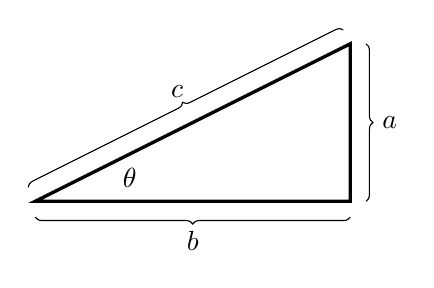
\begin{tikzpicture}
    \coordinate (C) at (0,2);
    \coordinate (D) at (4,2);
    \coordinate (E) at (4,4);
    \tkzMarkRightAngle(C,D,E)
    \tkzMarkAngle(D,C,E)
    \draw[decoration={brace,mirror,raise=.2cm},decorate,thin] (0,2)--(4,2);
    \draw[decoration={brace,mirror,raise=.2cm},decorate,thin] (4,2)--(4,4);
    \draw[decoration={brace,raise=.2cm},decorate,thin] (0,2)--(4,4);
    \draw[very thick] (D)--(E)--(C)--cycle;
    \node at (2,2-.5) {$b$};
    \node[] at (4+.5,3) {$a$};
    \node at (2-.2,3+.4) {$c$};
    \node at (1.2,2.3) {$\theta$};
  \end{tikzpicture}
\end{image}
We have that:
\[
a^2 + b^2 = c^2
\]
\end{theorem}


%The Pythagorean Theorem gives several key trigonometric identities.
%
%\begin{theorem}[Pythagorean Identities]\index{Pythagorean identities}
%  The following hold:
%  \[
%  \cos^2\theta+\sin^2\theta = 1 \qquad 1 + \tan^2\theta = \sec^2\theta \qquad \cot^2\theta + 1 = \csc^2\theta
%  \]
%  \begin{explanation}
%    From the unit circle we can see
%    \begin{image}
%\begin{tikzpicture}
%	\begin{axis}[
%            xmin=-1.1,xmax=1.1,ymin=-1.1,ymax=1.1,
%            axis lines=center,
%            width=4in,
%            ticks=none,
%            clip=false,
%            unit vector ratio*=1 1 1,
%            %xlabel=$x$, ylabel=$y$,
%            every axis y label/.style={at=(current axis.above origin),anchor=south},
%            every axis x label/.style={at=(current axis.right of origin),anchor=west},
%          ]        
%          \addplot [dashed, smooth, domain=(0:360)] ({cos(x)},{sin(x)}); %% unit circle
%
%          \addplot [textColor] plot coordinates {(0,0) (.766,.643)}; %% 40 degrees
%
%          \addplot [ultra thick,penColor] plot coordinates {(.766,0) (.766,.643)}; %% 40 degrees
%          \addplot [ultra thick,penColor2] plot coordinates {(0,0) (.766,0)}; %% 40 degrees
%          
%          %\addplot [ultra thick,penColor3] plot coordinates {(1,0) (1,.839)}; %% 40 degrees          
%
%          \addplot [textColor,smooth, domain=(0:40)] ({.15*cos(x)},{.15*sin(x)});
%          %\addplot [very thick,penColor] plot coordinates {(0,0) (.766,.643)}; %% sector
%          %\addplot [very thick,penColor] plot coordinates {(0,0) (1,0)}; %% sector
%          %\addplot [very thick, penColor, smooth, domain=(0:40)] ({cos(x)},{sin(x)}); %% sector
%          \node at (axis cs:.15,.07) [anchor=west] {$t$};
%          \node[penColor, rotate=-90] at (axis cs:.84,.322) {$\sin(t)$};
%          \node[penColor2] at (axis cs:.383,0) [anchor=north] {$\cos(t)$};
%          %\node[penColor3, rotate=-90] at (axis cs:1.06,.322) {$\tan(\theta)$};
%        \end{axis}
%\end{tikzpicture}
%    \end{image}
%    via the Pythagorean Theorem that
%    \[
%    \cos^2(t) + \sin^2(t) = 1.
%    \]
%    If we divide this expression by $\answer[given]{\cos^2(t)}$ we obtain
%    \[
%    1 + \tan^2(t) = \sec^2(t)
%    \]
%    and if we divide $\cos^2(t) + \sin^2(t) = 1$ by $\answer[given]{\sin^2(t)}$ we obtain
%    \[
%    \cot^2(t) + 1 = \csc^2(t).
%    \]
%  \end{explanation}
%\end{theorem}

We can simplify expressions that compose trig functions with inverse trig functions using the Pythagorean Theorem, as shown in the examples below. While these examples may seem a bit contrived at the moment, they will play a crucial role in an integration method featured in Calculus II.

\begin{example}
  Suppose that $\arctan(3/5) = \theta$. Compute $\sin(\theta)$. That is, compute $\sin(\arctan(3/5))$.
  \begin{explanation}
    If $\arctan(3/5) = \theta$, then $3/5=\tan(\theta)$.
%    \begin{align*}
%    \tan(\arctan(3/5)) &= \tan(\theta)\\
%    \answer[given]{3/5} &= \tan(\theta).
%    \end{align*}
    Now we will use the Pythagorean Theorem to deduce
If $\tan(\theta)=3/5$=opp/adj, the triangle in question must
    be similar to this triangle:
    \begin{image}[2in]
      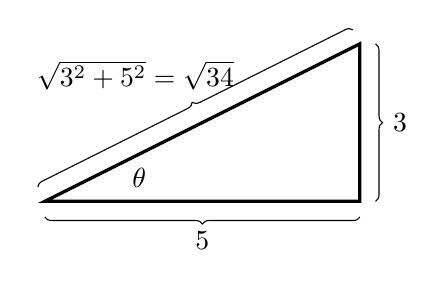
\begin{tikzpicture}
        \coordinate (C) at (0,2);
        \coordinate (D) at (4,2);
        \coordinate (E) at (4,4);
        \tkzMarkRightAngle(C,D,E)
        \tkzMarkAngle(D,C,E)
        \draw[decoration={brace,mirror,raise=.2cm},decorate,thin] (0,2)--(4,2);
        \draw[decoration={brace,mirror,raise=.2cm},decorate,thin] (4,2)--(4,4);
        \draw[decoration={brace,raise=.2cm},decorate,thin] (0,2)--(4,4);
        \draw[very thick] (D)--(E)--(C)--cycle;
        \node at (2,2-.5) {$5$};
        \node[anchor=west] at (4+.3,3) {$3$};
        \node at (2-.85,3+.6) {$\sqrt{3^2+5^2}=\sqrt{34}$};
        \node at (1.2,2.3) {$\theta$};
      \end{tikzpicture}
    \end{image}
    Notice that we filled in opp$=3$ and adj$=5$, then used the Pythagorean Theorem to compute the hypotenuse.
    From this triangle, we see that
    \[
    \sin(\theta) =\mbox{opp/hyp}= \answer[given]{3/\sqrt{34}}.
    \]
  \end{explanation}
\end{example}


\begin{example}
  Simplify
  \[
  \tan(\arccos(x))
  \]
  \begin{explanation}
 If
    \(
    \theta = \arccos(x)
    \)
    then $\tan(\arccos(x)) = \tan(\theta)$ and $\cos(\theta)=x=x/1$.
%    Apply cosine to both
%    sides of the equation above,
%    \begin{align*}
%      \cos(\theta) &= \cos(\arccos(x))\\
%      \cos(\theta) &= \answer[given]{x}.
%    \end{align*}
%    Now we will use the Pythagorean Theorem to deduce $\tan(\theta)$. 
If $\cos(\theta)=\mbox{adj/hyp}=x/1$, the triangle in question must
    be similar to this triangle below, which we assemble by filling in adj$=x$ and hyp$=1$, and using the Pythagorean Theorem to compute the opposite side.
    \begin{image}[2in]
      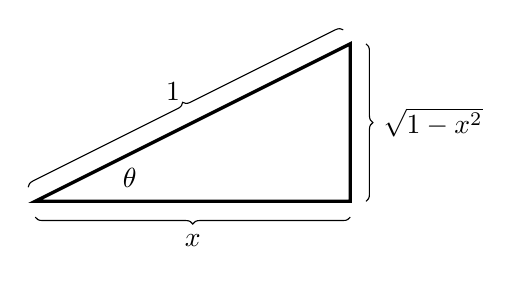
\begin{tikzpicture}
        \coordinate (C) at (0,2);
        \coordinate (D) at (4,2);
        \coordinate (E) at (4,4);
        \tkzMarkRightAngle(C,D,E)
        \tkzMarkAngle(D,C,E)
        \draw[decoration={brace,mirror,raise=.2cm},decorate,thin] (0,2)--(4,2);
        \draw[decoration={brace,mirror,raise=.2cm},decorate,thin] (4,2)--(4,4);
        \draw[decoration={brace,raise=.2cm},decorate,thin] (0,2)--(4,4);
        \draw[very thick] (D)--(E)--(C)--cycle;
        \node at (2,2-.5) {$x$};
        \node[anchor=west] at (4+.3,3) {$\sqrt{1-x^2}$};
        \node at (2-.25,3+.4) {$1$};
        \node at (1.2,2.3) {$\theta$};
      \end{tikzpicture}
    \end{image}
    From this triangle, we see that
    \[
    \tan(\arccos(x)) = \tan(\theta) = \mbox{opp/adj}=\answer[given]{\frac{\sqrt{1-x^2}}{x}}.
    \]
  \end{explanation}
\end{example}

\subsection{Learning Objectives}
After completing this section, students should be able to:
\vspace{.05in}

\noindent$\bullet$ Know the domain and range of the inverse trig functions.
\\$\bullet$ Evaluate inverse trigonometric functions of standard values.
\\$\bullet$ Simplify expressions involving trigonometric functions and inverse trigonometric functions.

%\outcome{Know the domains and ranges of the inverse trigonometric functions.}
%\outcome{Evaluate inverse trigonometric functions of standard values.}
%\outcome{Understand the relationship between trigonometric and inverse trigonometric functions.}
%\outcome{Evaluate expressions and solve equations involving
%          trigonometric functions and inverse trigonometric functions.}






\end{document}